% $HeadURL$

%%%%%%%%%%%%%%%%%%%%%%%%%%%%%%%%%%%%%%%%%%%%%%%%%%%%%%%%%%%%%%%%%%%%%%
%%                     Production
%%%%%%%%%%%%%%%%%%%%%%%%%%%%%%%%%%%%%%%%%%%%%%%%%%%%%%%%%%%%%%%%%%%%%%

\paragraph{Glyph: \glyph{Production}}\label{sec:production}

\glyph{Production} is the arc used to represent the fact that an entity pool is 
produced by a process. In the case of a reversible process, the 
\glyph{production} arc also acts as a \glyph{consumption} arc.

\begin{glyphDescription}
 \glyphSboTerm SBO:0000393 ! production.
 \glyphOrigin Any \glyph{process node} (\sect{PNs}).
 \glyphTarget Any \glyph{EPN} (\sect{EPNs}).
 \glyphEndPoint The target extremity of a \glyph{production} carries a filled arrowhead.
 \end{glyphDescription}

A cardinality label can be associated with a \glyph{production} arc indicating the stoichiometry of a process.

\begin{figure}[H]
  \centering
  \includegraphics[scale = 0.4]{images/production}
  \caption{The \PD glyph for \glyph{production}.}
  \label{fig:production}
\end{figure}

\fig{prod-card} illustrates the use of consumption/production arc cardinality labels to represent the stoichiometry of a process.

\begin{figure}[H]
  \centering
  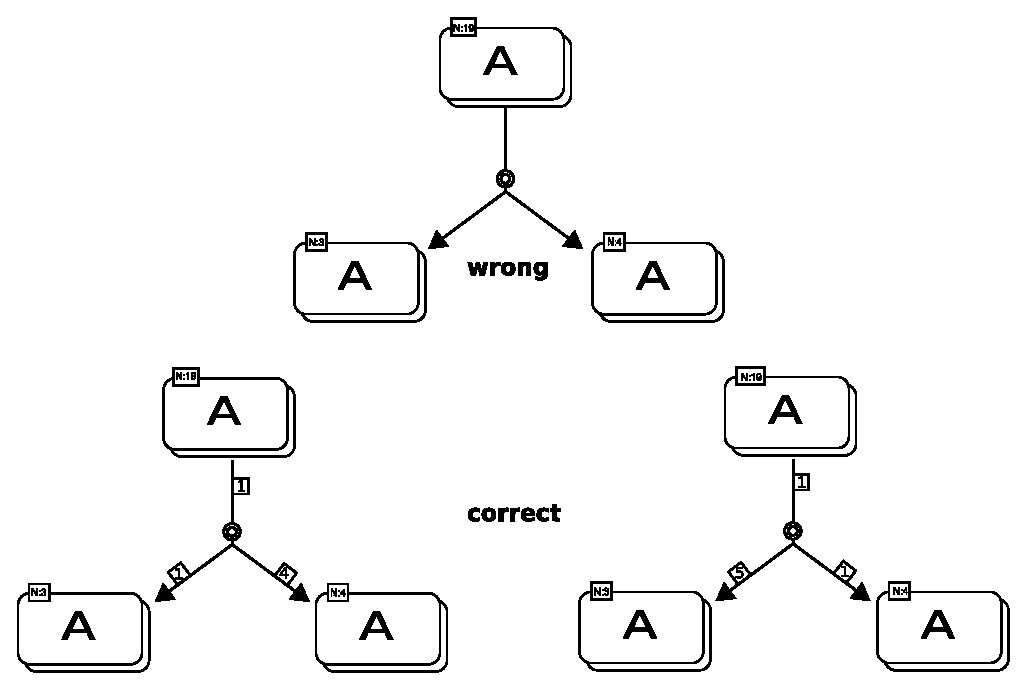
\includegraphics[scale = 0.85]{examples/stoichEx1}
  \caption{Cardinality for production arcs.}
  \label{fig:prod-card}
\end{figure}




% The following is for [X]Emacs users.  Please leave in place.
% Local Variables:
% TeX-master: "../sbgn_PD-level1"
% End:

